\documentclass[11pt,a4paper]{article}

\usepackage[utf8]{inputenc}
\usepackage[T1]{fontenc}
\usepackage[margin=0.8in]{geometry}
\usepackage{enumitem,titlesec,cite}
\usepackage{booktabs}
\usepackage{tikz}
\usetikzlibrary{arrows.meta, positioning}
\usepackage[hidelinks]{hyperref}

\titlespacing*{\section}{0pt}{10pt}{4pt}
\setlist[itemize]{noitemsep, topsep=3pt, leftmargin=1.4em}
\setlist[enumerate]{noitemsep, topsep=3pt, leftmargin=1.4em}

\title{\vspace{-1.5em}\textbf{Predictive Runtime Protection for Distributed Real-Time AI Systems}}
\author{
Mayur Raju (24BCS073) \quad P Gnandeep (24BCS095) \quad P Maruthi (24BCS098) \\
P Sanjay (24BCS100) \quad S Sudharsan Reddy (24BCS130) \\
[1ex]
\textit{Department of Computer Science and Engineering} \\
\textit{Course: Real-Time Systems} \\
\textit{Instructor: Dr.~Swagatika Sahoo}
}
\date{}

\begin{document}
\maketitle

\begin{abstract}
\noindent
Real-time AI pipelines on distributed edge platforms must complete multi-stage inference within firm deadlines, yet their execution times fluctuate due to resource contention, thermal throttling, and wireless network variability. Many scheduling and placement policies act only after queues saturate or overruns are observed, at which point the remaining slack may be smaller than the network transfer time required to offload the computation. This project proposes a proactive runtime protection architecture that uses a compact Graph Neural Network (GNN) to estimate deadline-miss risk from runtime task dependencies and resource queues. Based on this risk, the system arbitrates between local execution, cooperative offloading to a neighboring device, and degraded local fallback. In addition to offline model alternatives, degraded execution incorporates in-flight early exit: when waiting for remaining layers or iterations threatens a deadline violation, ongoing computation is truncated at the latest valid structural boundary and committed immediately. A background Federated Learning component maintains remote execution-latency and reliability estimates without centralizing raw telemetry, and Response Time Analysis is applied to verify schedulability under worst-case interference. The framework is evaluated in a discrete-event simulation of a heterogeneous multi-robot mesh against standard real-time baselines including FIFO, Rate Monotonic, Earliest Deadline First, unconditional offloading, and reactive degradation.
\end{abstract}

\section{Motivation for Selecting the Topic}
Real-time AI systems---such as autonomous drones, self-driving vehicles, mobile robots, and surveillance nodes---execute multi-stage machine learning pipelines under firm timing constraints. In these systems, delayed computation can be catastrophic, rendering even high-accuracy inference results useless.

In distributed edge environments, execution times vary due to dynamic inputs, thermal throttling, hardware contention, and wireless channel jitter. Many scheduling and offloading policies respond after local queues back up or latency degradation is observed. By that point, the remaining time buffer (slack) may be smaller than the network transmission delay, leaving few options for recovery.

This project examines proactive, low-overhead runtime intervention as an alternative. By using a lightweight predictive model to identify impending deadline violations early, the system gains the lead time needed to choose among local execution, cooperative neighbor offloading, and degraded local fallback. The framework is designed generically for distributed real-time AI pipelines, using a heterogeneous fleet of drones and ground robots as the evaluation environment.

\section{Problem Statement}
When an edge device executing dependent real-time tasks experiences a sudden compute overload, relying exclusively on local processing risks deadline violations. Offloading redistributes workload, but network latency variation and remote queue states introduce uncertainty. Static redundant replication improves fault tolerance but incurs significant compute and energy overheads on resource-constrained devices.

Existing literature independently explores predictive deadline detection, graph-based offloading, federated learning for edge nodes, and redundant execution. This project studies their integration into a unified runtime arbitration policy. The core research question is:
\begin{quote}
\textit{Can a lightweight, graph-based predictive model anticipate deadline misses early enough to dynamically arbitrate between local execution, cooperative offloading, and degraded fallback, while keeping decision-making overhead small enough to preserve task schedulability?}
\end{quote}

\section{Project Objectives}
\begin{enumerate}
    \item Represent multi-stage AI tasks, dependencies, execution times, and end-to-end deadlines as Directed Acyclic Graphs.
    \item Train a compact Graph Neural Network on runtime graph states to output deadline-violation risk within a bounded, measured inference budget.
    \item Apply Federated Learning (FedAvg) as a background activity to maintain remote execution-latency and node reliability estimates without centralizing raw telemetry.
    \item Design a runtime arbitration policy that selects between local execution, cooperative offload, and degraded fallback based on predicted risk and task criticality.
    \item Incorporate a mid-execution early-exit mechanism that evaluates the risk of waiting and dynamically commits partial valid inference outputs when full generation would breach timing constraints.
    \item Apply Response Time Analysis to examine whether degraded execution modes remain schedulable under worst-case higher-priority interference.
    \item Benchmark the framework in a discrete-event simulation against FIFO, Rate Monotonic, Earliest Deadline First, unconditional offloading, and reactive baselines.
\end{enumerate}

\section{Literature Review}

\textbf{Enhancing Deadline Miss Early Detection for DAG Tasks with Variable Probabilistic Thresholds} \cite{paper_toba2026}:\\
Toba, Baruah, and Azumi model autonomous-driving perception pipelines as DAG tasks subject to execution-time variation, using probabilistic execution times rather than worst-case assumptions to compute per-node time constraints, which reduces the pessimism of earlier early-detection methods. The contribution is analytical and diagnostic: it quantifies the possibility of a deadline miss at node release, without specifying a runtime recovery mechanism.

\medskip
\textbf{SeReMAS: Self-Resilient Mobile Autonomous Systems Through Predictive Edge Computing} \cite{paper_callegaro2021}:\\
Callegaro, Levorato, and Restuccia propose a data-driven framework that dispatches redundant task replicas to edge servers to improve task execution probability under uncertain wireless channels. A Deep Reinforcement Learning predictor selects task assignments from application-, network-, and telemetry-based features, and the system is prototyped on a drone with a Jetson Nano and multiple WiFi interfaces. The predictor is trained centrally over a fixed set of servers and channels.

\medskip
\textbf{Edge-Based QoS-Aware Adaptive Task Placement: A Closed-Loop Control in Multi-Robot Systems} \cite{paper_tran2026}:\\
Tran et al.\ evaluate local execution, static offloading, and adaptive placement across networked robots under CPU and channel contention. Their closed-loop controller scores placements using measured latency, CPU utilization, and switching overhead observed over recent time windows, responding to observed degradation rather than to a forecast of upcoming bottlenecks.

\medskip
\textbf{Federated Graph Neural Networks for Dynamic Computation Offloading in Vehicular Networks} \cite{paper_xu2024}:\\
Xu et al.\ propose V-FedGNN, embedding vehicle speed, location, available resources, and wireless conditions into a graph structure and combining Federated Learning with a GNN to minimize weighted computation offloading delay across vehicle nodes. The reported objectives are offloading prediction accuracy and reduced offloading latency rather than firm per-task deadline satisfaction.

\section{Comparison of Existing Work and Proposed Work}

\begin{table}[htbp]
\centering
\caption{Comparison Between Related Works and Proposed Architecture}
\label{tab:comparison}
\vspace{4pt}
\small
\begin{tabular}{p{3.1cm}p{1.9cm}p{1.8cm}p{1.6cm}p{1.6cm}p{3.2cm}}
\toprule
\textbf{Work} & \textbf{Prediction} & \textbf{Graph / GNN} & \textbf{Federated} & \textbf{Offload} & \textbf{Execution Strategies} \\
\midrule
Toba et al.\ \cite{paper_toba2026}    & Analytical    & DAG model & No  & No  & Detection only \\
SeReMAS \cite{paper_callegaro2021}    & Learned (DRL) & No        & No  & Yes & Replication \\
Tran et al.\ \cite{paper_tran2026}   & Measured state& No        & No  & Yes & Local / offload \\
V-FedGNN \cite{paper_xu2024}         & Learned       & Yes       & Yes & Yes & Offload latency objective \\
\textbf{Proposed}                    & Learned (GNN) & Yes       & Yes & Yes & Local / offload / early-exit degraded \\
\bottomrule
\end{tabular}
\end{table}

\noindent
The surveyed works address these elements separately: analytical detection identifies impending misses without specifying a recovery action; measurement-driven placement acts on observed degradation; and the federated graph framework optimizes offloading latency rather than per-task deadline satisfaction. This project studies their integration into a single runtime arbitration policy that evaluates predicted risk and selects an execution mode accordingly, while treating decision overhead as a measured quantity constrained by the available slack.

\section{Architecture Overview}

The framework runs as a predictive decision loop across an edge mesh, shown in Figure~\ref{fig:architecture}.

\begin{figure}[htbp]
\centering
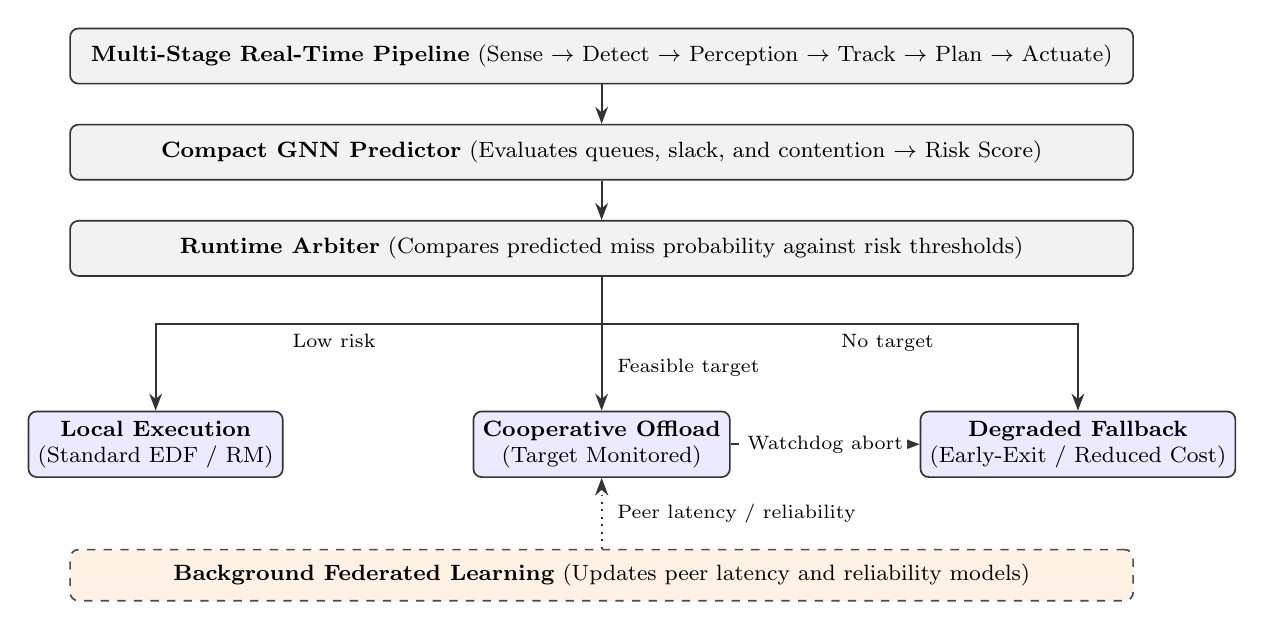
\begin{tikzpicture}[
    >=Stealth,
    node distance=0.5cm,
    font=\footnotesize,
    stage/.style={rectangle, draw=black!80, fill=gray!10, rounded corners=3pt, minimum width=13.5cm, minimum height=0.7cm, align=center, line width=0.6pt},
    opt/.style={rectangle, draw=black!80, fill=blue!8, rounded corners=3pt, minimum width=2.9cm, minimum height=0.8cm, align=center, line width=0.6pt},
    fl/.style={rectangle, draw=black!70, dashed, fill=orange!10, rounded corners=3pt, minimum width=13.5cm, minimum height=0.65cm, align=center, line width=0.6pt},
    arrow/.style={->, line width=0.7pt, draw=black!80}
]

\node[stage] (pipeline) {\textbf{Multi-Stage Real-Time Pipeline} (Sense $\to$ Detect $\to$ Perception $\to$ Track $\to$ Plan $\to$ Actuate)};
\node[stage, below=of pipeline] (gnn) {\textbf{Compact GNN Predictor} (Evaluates queues, slack, and contention $\to$ Risk Score)};
\node[stage, below=of gnn] (arbiter) {\textbf{Runtime Arbiter} (Compares predicted miss probability against risk thresholds)};

\node[opt, below=1.7cm of arbiter] (offload) {\textbf{Cooperative Offload}\\(Target Monitored)};
\node[opt, left=2.4cm of offload] (local) {\textbf{Local Execution}\\(Standard EDF / RM)};
\node[opt, right=2.4cm of offload] (degraded) {\textbf{Degraded Fallback}\\(Early-Exit / Reduced Cost)};

\node[fl, below=0.9cm of offload] (federated) {\textbf{Background Federated Learning} (Updates peer latency and reliability models)};

\draw[arrow] (pipeline) -- (gnn);
\draw[arrow] (gnn) -- (arbiter);

\draw[line width=0.7pt, draw=black!80] (arbiter.south) -- ++(0,-0.6) coordinate (j);
\draw[arrow] (j) -| node[pos=0.3, below, font=\scriptsize] {Low risk} (local.north);
\draw[arrow] (j) -- node[right=2pt, font=\scriptsize] {Feasible target} (offload.north);
\draw[arrow] (j) -| node[pos=0.3, below, font=\scriptsize] {No target} (degraded.north);

\draw[arrow, dashed, line width=0.75pt] (offload.east) -- node[font=\scriptsize, fill=white, inner sep=1.5pt] {Watchdog abort} (degraded.west);

\draw[arrow, dotted, line width=0.75pt] (federated.north) -- node[right=2pt, font=\scriptsize] {Peer latency / reliability} (offload.south);

\end{tikzpicture}
\caption{Overview of the runtime protection workflow. The GNN estimates risk from pipeline and queue states, the arbiter dispatches the task to local execution, cooperative offloading, or degraded fallback, and background federated learning maintains peer performance estimates.}
\label{fig:architecture}
\end{figure}

\textbf{Simulation layer.} A millisecond-resolution discrete-event simulator models heterogeneous devices (drones, ground robots, and edge servers) with shared CPU/GPU queues, thermal throttling, and wireless channel jitter. The workload is an autonomous AI pipeline consisting of sensing, obstacle detection, perception, tracking, path planning, and actuation stages. Each stage has a defined period, priority, deadline, nominal execution budget, and degraded fallback budget. The simulator tracks dynamic slack, measured as the remaining time before a task's deadline minus its expected execution time.

\textbf{Prediction layer.} At each scheduling checkpoint, the current system state is mapped to a graph in which nodes represent active tasks and hardware execution queues, and edges denote data dependencies and resource contention. A compact two-layer Graph Neural Network processes this graph to output a deadline-miss probability and to indicate the primary resource bottleneck (for example, GPU queue saturation or thermal throttling). Inference cost is measured and reported as scheduler overhead relative to the available slack, and is treated as a budgeted quantity rather than assumed negligible.

\textbf{Federated layer.} A lightweight model maps device profiles and channel states to predicted remote execution latency and peer reliability. Nodes update this model locally from completed tasks and aggregate weights periodically using Federated Averaging (FedAvg), exchanging only parameter updates. Aggregation is scheduled as a background, best-effort activity off the task dispatch path, so that runtime decisions always use the currently available local copy of the model; the residual interference of this background activity on foreground tasks is itself a quantity to be measured rather than assumed to be zero.

\textbf{Arbitration layer.} When a task arrives, the arbiter checks the predicted miss probability. Low-risk tasks run locally under standard scheduling. If deadline risk is high, the arbiter checks whether an eligible neighbor can receive, process, and return the task within the deadline margin. Tasks sent over the network remain under watchdog supervision; if the remote device encounters unexpected contention, the system aborts the offload and handles the task locally.

\textbf{Verification layer.} If no neighbor is eligible or an offload is aborted, the system activates a degraded local fallback mode with a reduced execution budget. Beyond switching to pre-configured lightweight models, degraded execution incorporates in-flight early exit: ongoing iterative or layer-wise inference tasks are evaluated mid-execution against the remaining slack budget. If continuing computation would exceed the hard deadline, the runtime interrupts execution at the latest structurally valid stage and immediately commits the partial output. These fallback boundaries are analyzed using exact Response Time Analysis for fixed-priority preemptive scheduling, establishing that the truncated execution budgets satisfy task deadlines under worst-case local interference.

\section{Tools and Evaluation}
The software stack uses Python 3 with PyTorch and PyTorch Geometric for GNN modeling, NetworkX for runtime graph structures, a custom FedAvg module, and a discrete-event simulation core. No external datasets are needed; workloads and contention patterns are procedurally generated by the simulator, using distinct random seeds for training and testing.

Evaluation metrics include total and critical deadline-miss ratios, worst-case and average response times, response-time jitter, offload success rate, fallback and early-exit activation count, and GNN inference overhead relative to available slack. The evaluation examines the trade-off between deadline reliability and the additional computational and communication cost incurred to achieve it.

\section{Scope and Limitations}
Experiments are conducted within a discrete-event simulator that models CPU/GPU queues, preemption, thermal throttling, and channel delays, but abstracts aerodynamic dynamics, physical RF multipath fading, and low-level cache interference. Federated learning is evaluated across simulated clients rather than physical hardware. Timing results therefore hold under these modelled resource and interference assumptions and are reported as such.

\begin{thebibliography}{9}

\bibitem{paper_toba2026}
H.~Toba, S.~Baruah, and T.~Azumi,
``Enhancing Deadline Miss Early Detection for DAG Tasks with Variable Probabilistic Thresholds,''
\textit{ACM Transactions on Embedded Computing Systems}, Just Accepted, 2026.
\newblock DOI: \href{https://doi.org/10.1145/3808694}{10.1145/3808694}.

\bibitem{paper_callegaro2021}
D.~Callegaro, M.~Levorato, and F.~Restuccia,
``SeReMAS: Self-Resilient Mobile Autonomous Systems Through Predictive Edge Computing,''
in \textit{Proc.\ 18th Annual IEEE Int.\ Conf.\ on Sensing, Communication, and Networking (SECON)},
pp.~1--9, 2021.
\newblock DOI: \href{https://doi.org/10.1109/SECON52354.2021.9491618}{10.1109/SECON52354.2021.9491618}.

\bibitem{paper_tran2026}
T.~Tran, J.~Kua, T.~N.~Hoang, M.~Tran, H.~Lyu, and J.~Jin,
``Edge-Based QoS-Aware Adaptive Task Placement: A Closed-Loop Control in Multi-Robot Systems,''
\textit{arXiv preprint arXiv:2606.00552}, 2026.

\bibitem{paper_xu2024}
Y.~Xu, Y.~Lu, Y.~Dai, C.~Sun, J.~Liu, and W.~Zhang,
``Federated Graph Neural Networks for Dynamic Computation Offloading in Vehicular Networks,''
in \textit{GLOBECOM 2024 -- 2024 IEEE Global Communications Conference},
Cape Town, South Africa, Dec.\ 2024.
\newblock DOI: \href{https://doi.org/10.1109/GLOBECOM52923.2024.10901545}{10.1109/GLOBECOM52923.2024.10901545}.

\end{thebibliography}

\end{document}
